\chapter{Performance}

When working with interactive visualizations, performance plays a crucial role in ensuring a smooth user experience, especially as datasets grow larger and more complex. With increasing data points and variables, the demand for both computational power and efficient rendering becomes essential. Interactive visualizations can encounter performance bottlenecks due to factors such as data size, rendering techniques, bandwidth, and hardware limitations. As data size increases, performance issues can manifest in the form of delayed rendering, increased memory usage, and ultimately, a sluggish or unresponsive interface. These challenges make it essential to understand and implement performance-enhancing solutions such as tiling, level of detail (LOD) management, GPU acceleration, and hierarchical data organization.

In this context, two experiments were conducted to benchmark and understand the performance implications of interactive visualizations, both in terms of data size and choice of visualization libraries. The following sections analyze these experiments, where Figure \ref{fig:performance1} and Figure \ref{fig:performance2} showcase the performance metrics obtained.

\section{Experiment 1: Impact of Data Size}

\begin{figure}[H]
    \centering
    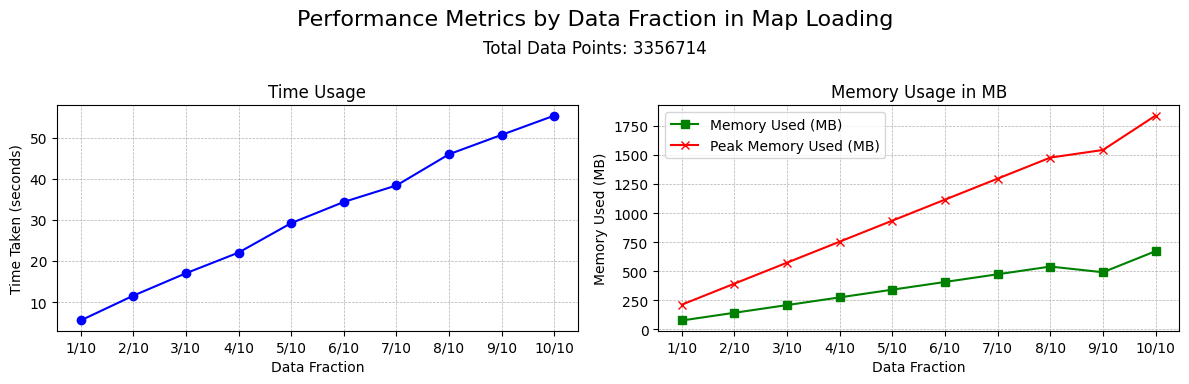
\includegraphics[width=0.8\textwidth]{figures/map_performance.png}
    \caption{Performance metrics for incremental data loading in a map visualization.}
    \label{fig:performance1}
\end{figure}    

Figure \ref{fig:performance1} illustrates the performance metrics captured when incrementally loading fractions of a dataset into a map visualization. In this experiment, each data point represented a bird observation in Sweden, and fractions of the dataset were loaded from 1/10th up to the entire dataset (10/10ths, or 3'356'714 observations). Two metrics were recorded: Time Usage (in seconds) and Memory Usage (in MB).

\subsection{Time Usage Analysis}

The left subplot of \ref{fig:performance1} shows a linear trend in time consumption as the data fraction increases. The time taken rises from approximately 10 seconds for 1/10th of the data to over 50 seconds for the entire dataset. This trend reflects the computational load associated with managing and rendering larger datasets in real-time.

This increase in time usage can be attributed to the overhead of both loading data into memory and the rendering process itself. With each increment, the visualization needs to plot more points on the map, which places a growing strain on both the CPU and GPU, depending on the level of interactivity and graphical requirements.

\subsection{Memory Usage Analysis}

The right panel of Figure 1 captures memory usage with two lines: one for Memory Used and another for Peak Memory Used. Memory Used remains relatively lower, while Peak Memory steadily climbs with each data increment.

The growing gap between regular and peak memory usage can be attributed to the temporary memory required to process the data before rendering. As the data size increases, the visualization needs to allocate more temporary memory for computation, even if the plotted memory stabilizes.

This memory trend suggests that managing data efficiently, such as by tiling or downsampling, could reduce the memory load, making the visualization more responsive without compromising on detail.

\section{Experiment 2: Impact of Plotting Library on Performance}

\begin{figure}[H]
    \centering
    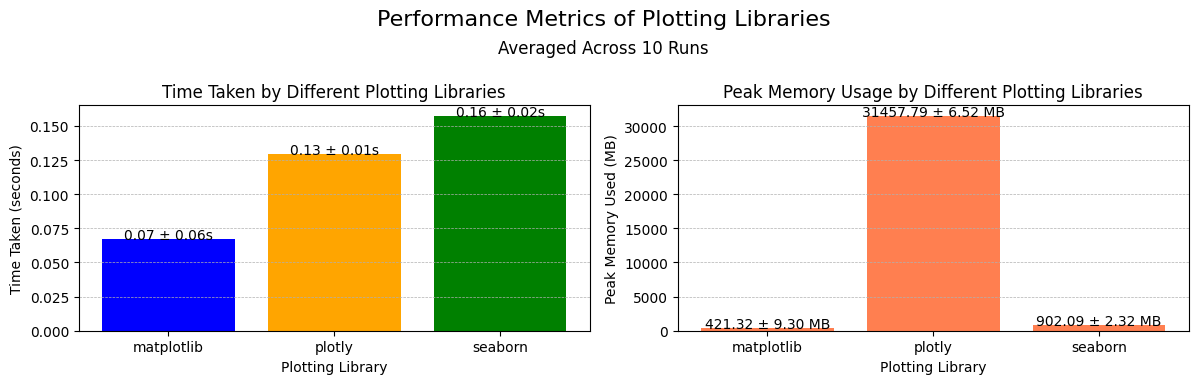
\includegraphics[width=0.8\textwidth]{figures/barplot_performance.png}
    \caption{Performance metrics for different plotting libraries.}
    \label{fig:performance2}
\end{figure}

In Figure \ref{fig:performance2}, the performance of three plotting libraries—Matplotlib, Plotly, and Seaborn—was measured by plotting the frequency of the 10 most common bird species in Sweden. To ensure accuracy and confidence in the results, each test was run 10 times, and the Time Taken and Peak Memory Usage metrics were averaged across these runs, with standard deviations included to quantify variability.

\subsection{Time Taken Analysis}

The left panel of Figure \ref{fig:performance2} shows that Matplotlib remains the fastest library, with an average time of 0.07 seconds ± 0.06 seconds. Plotly and Seaborn, however, took considerably longer, with average times of 0.14 seconds ± 0.02 seconds for Plotly and 0.15 seconds ± 0.01 seconds for Seaborn.

The high standard deviation for Matplotlib indicates some variability in its runtime, possibly due to fluctuations in processing lower-level operations. In contrast, Plotly and Seaborn show relatively stable performance with smaller standard deviations, reflecting their structured approach to rendering but at the cost of increased processing time.

Matplotlib's efficiency is likely due to its streamlined focus on static plotting, while Plotly's interactivity and Seaborn's additional styling complexity add to their time overhead. These findings emphasize that while Matplotlib is optimal for static visualizations, Plotly and Seaborn introduce extra time due to their functionality and aesthetic layers, respectively.

\subsection{Memory Usage Analysis}

The right panel of Figure \ref{fig:performance2} reveals a stark contrast in peak memory usage among the libraries. Plotly uses significantly more memory, averaging 31,471.73 MB ± 40.09 MB, highlighting the high cost of interactivity. Seaborn requires considerably less memory, averaging 903.09 MB ± 2.13 MB, and Matplotlib remains the most memory-efficient, with an average of 422.25 MB ± 9.62 MB.

The consistent but high memory usage for Plotly suggests that its interactive features, such as hover and zoom functionality, impose a substantial memory footprint. These features, while enhancing user engagement, demand extensive resources for rendering and data management, particularly when handling large datasets or complex visualizations.

Seaborn, despite being built on top of Matplotlib, requires additional memory to manage stylistic elements. Matplotlib's low memory usage reaffirms its suitability for static visualizations where memory constraints are critical. This suggests that when designing interactive visualizations with large datasets, it is essential to account for Plotly's memory requirements, while Matplotlib and Seaborn serve as better choices for simpler plots.